\documentclass{article}
\usepackage{graphicx}
\usepackage{enumitem}
\usepackage{pdfpages}
\usepackage[a4paper, left=1in, right=1in, top=1in, bottom=1in]{geometry}
\usepackage[english]{babel}
\usepackage{fancyhdr}
\pagestyle{fancy}

% Header
\fancyhead[L]{Niklas Fister}
\fancyhead[C]{Kantonnschule Wettingen - English}
\fancyhead[R]{\thepage}


% clear Footer
\fancyfoot{}

% Title
\title{\Huge\textbf{English Essay}}
\author{Niklas Fister}
\date{\today}

\begin{document}
\maketitle
\thispagestyle{empty}
\newpage

\section{Important Information}
\begin{itemize}[parsep=0pt]
    \item Don't be distracted by the word 'Discuss'. It just mean your Essay needs to be the discussion and you need to show your opinion.
    \item The 'Why'-scentence under the Stantement (the idea for an stantement/idea).
    \item Teachers know what the statemnt says, but it should be clear, what topic it is; don't have to put in the entire quote, but the meaning of it should be clear.
    \item You can say: While one of these thing might be true, this is the reason to be against it.
\end{itemize}
\newpage

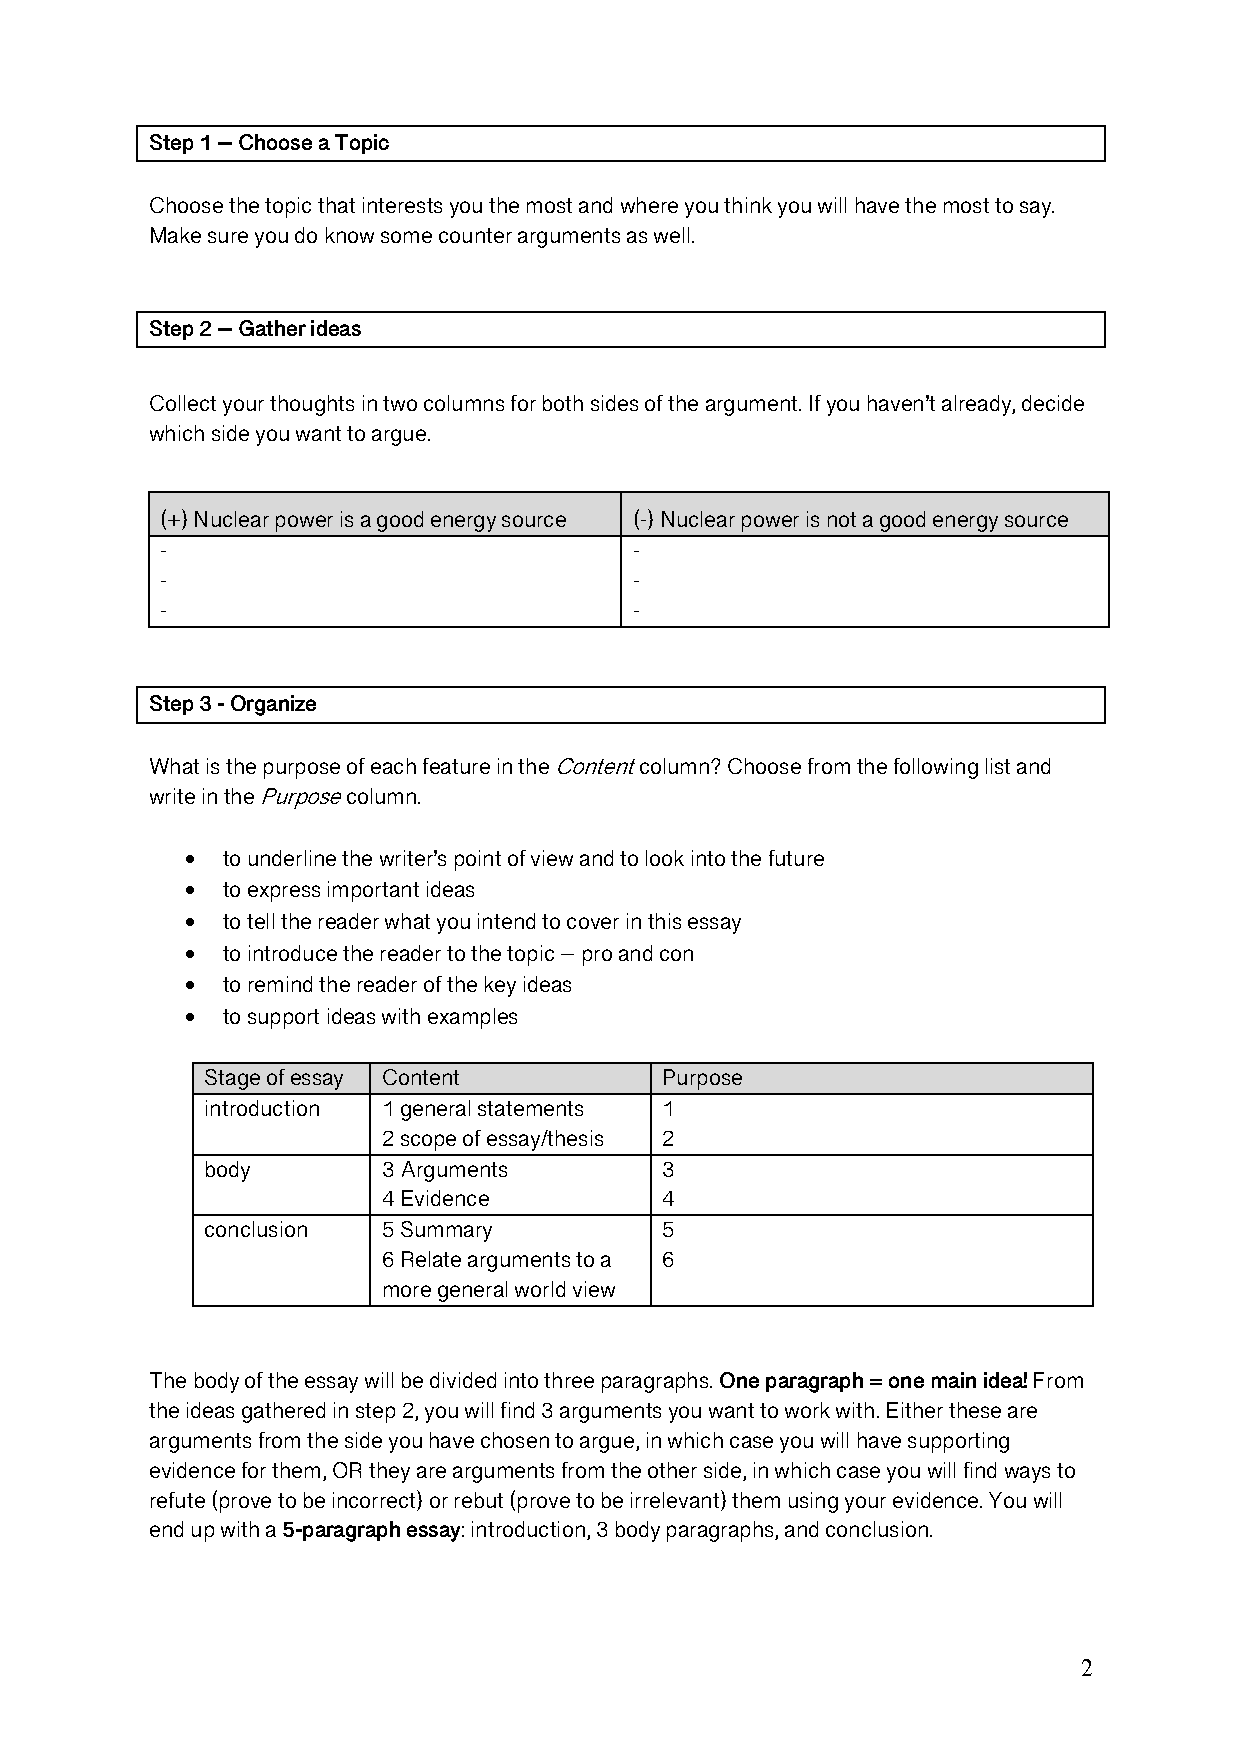
\includepdf[nup=2x2, scale=0.8, pages=-]{resources/pdf/Argumentative Essay Writing.pdf}

\section{Essay with GPT}
\textbf{German Politics: Balancing Tradition and Modern Challenges}

The political system of Germany, with its strong democratic foundation, has long been a model of stability and progress in Europe. As the country faces growing challenges—from climate change to social inequality—the need for political reform and innovation becomes more pressing. This essay explores the current political landscape of Germany and examines how it can adapt to meet contemporary demands without compromising its foundational principles.

One of the strengths of German politics lies in its federal system, which ensures regional representation and balances power between the national and state governments. This structure enables local governments to tailor policies to their specific needs, fostering innovation and inclusivity. For example, Germany's Energiewende (energy transition) initiative has allowed individual states like Bavaria to implement renewable energy policies suited to their local resources. However, critics argue that this decentralized approach sometimes slows national decision-making, particularly in urgent matters like climate action. Therefore, while federalism provides diversity and representation, it also demands stronger coordination at the national level to address overarching issues effectively.

Another cornerstone of German politics is its coalition-based governance, which ensures that a wide range of political perspectives is represented in policymaking. By requiring parties to collaborate, coalitions promote compromise and discourage extreme partisanship. The current traffic light coalition—comprising the Social Democrats (SPD), Greens, and Free Democrats (FDP)—illustrates this principle by addressing diverse priorities such as environmental sustainability and economic growth. However, coalition politics can also lead to gridlock, as conflicting party interests may hinder decisive action. For instance, debates over climate measures and fiscal policy often delay reforms. Thus, while coalition governance fosters inclusivity, it needs mechanisms to streamline decision-making for critical reforms.

Germany's approach to social policies reflects its commitment to equity and welfare, making it a leader in areas such as healthcare, education, and workers’ rights. Programs like universal healthcare and vocational training demonstrate the government’s dedication to social justice. Yet, these systems face challenges, including an aging population and increasing financial strain. Critics warn that without reform, these systems may become unsustainable. Policymakers must balance maintaining high standards of social support with ensuring their long-term viability, emphasizing innovation and efficiency.

In conclusion, German politics is defined by its commitment to democracy, regional representation, coalition-building, and social equity. While these elements have been instrumental in fostering stability and progress, they also present challenges in an era of rapid change and global uncertainty. To remain effective, Germany must adapt its political structures and policies while preserving its democratic ideals. Ultimately, the strength of German politics lies in its ability to evolve, ensuring that it continues to serve its citizens and set an example for the world. Through thoughtful reform and collaboration, Germany can address modern challenges without compromising its core values.

\newpage
\section{Essay without GPT}
\textbf{Political Strugle: The balance between seperation and integration of different cultures}

The act of integration has always been a difficult topic and finding the balance hardly possible. While the right in politics is against the integration, the left wants to include them entirely. Some are afraid to loose their own cultures in the act of intigration and others want just that.


\end{document}